\documentclass[tikz,border=10pt]{standalone}
\begin{document}
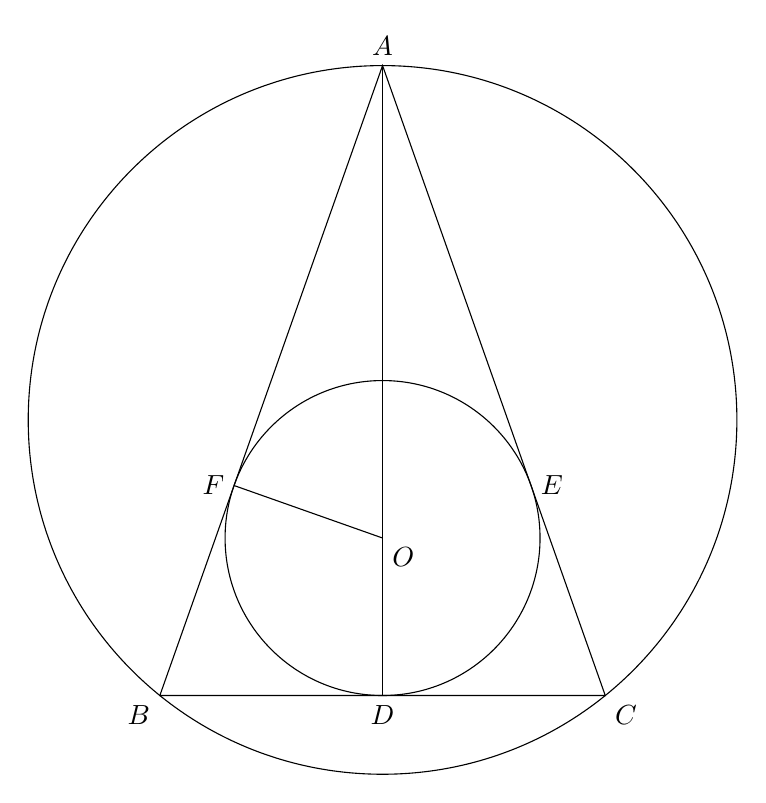
\begin{tikzpicture}
    \coordinate (A) at (0,6);
    \coordinate (B) at (-2.8284, -2);
    \coordinate (C) at (2.8284, -2);
    \coordinate (D) at (0,-2);
    \coordinate (E) at (1.8856, 0.6667);
    \coordinate (F) at (-1.8856, 0.6667);
    \coordinate (O) at (0,0);
    \coordinate (K) at (0, 1.5);

    \draw (K) circle (4.5);
    \draw (O) circle (2);
    \draw (A) -- (B) -- (C) -- cycle;
    \draw (A) -- (D);
    \draw (O) -- (F);

    \node[above] at (A) {$A$};
    \node[below left] at (B) {$B$};
    \node[below right] at (C) {$C$};
    \node[below] at (D) {$D$};
    \node[right] at (E) {$E$};
    \node[left] at (F) {$F$};
    \node[below right] at (O) {$O$};
\end{tikzpicture}
\end{document}
